\documentclass[12pt,a4paper,oneside,titlepage]{report}
\usepackage[T1]{fontenc}
\usepackage[latin1]{inputenc}
\usepackage[italian]{babel}


   %%%%%%%%%%%%%%%%%%%%%%%%%%%%%%%%%%%%%%%%%%%%%%%%%%%%%%%%%
\usepackage{frontespizio}
% Col pacchetto tocbibind compariranno nell'indice anche
% la bibliografia ed eventualmente l'indice analitico
\usepackage[nottoc]{tocbibind}

% Il pacchetto indentfirst abolisce la fastidiosa convenzione
% anglosassone di fa cominciare la prima riga di un
% capitolo o sezione a margine sinistro, senza rientro:
\usepackage{indentfirst}

%\usepackage{graphicx} % gia' caricato da uniudtesi
%\graphicspath{{./figure/}}
%\usepackage{epstopdf}

 %%%%%%%%%%%%%%%%%%%%%%%%%%%%%%%%%%%%%%%%%%%%%%%%

\usepackage{amsmath,amsfonts,amssymb,amsthm}
\usepackage{latexsym}


%%%%%%%%%%%%%%%%%%%%%%%%%%%%%%%%%%%%%%%%%%%%%%%%%%%%%%%


   %%%%%%%%%%%%%%%%%%%%%%%%%%%%%%%%%%%%%%%%%%%

\newcommand{\N}{\mathbb{N}}
\newcommand{\Z}{\mathbb{Z}}
\newcommand{\K}{\mathbb{K}}
\newcommand{\R}{\mathbb{R}}
\newcommand{\C}{\mathbb{C}}
\newcommand{\A}{\mathbb{A}}
\newcommand{\I}{\mathbb{I}}

   %%%%%%%%%%%%%%%%%%%%%%%%%%%%%%%%%%%%%%%%%%%%

\DeclareMathOperator{\traccia}{tr}
\DeclareMathOperator{\sen}{sen}
\DeclareMathOperator{\cl}{cl}
\DeclareMathOperator{\dom}{dom}
\DeclareMathOperator{\dist}{dist}
\DeclareMathOperator{\arcsen}{arcsen}
\DeclareMathOperator*{\maxlim}{max\,lim}
\DeclareMathOperator*{\minlim}{min\,lim}
\DeclareMathOperator*{\deepinf}{\phantom{\makebox[0pt]{p}}inf}

    %%%%%%%%%%%%%%%%%%%%%%%%%%%%%%%%%%%%%%%%%%%%

\newcommand{\varsum}[3]{\sum_{#2}^{#3}\!
   {\vphantom{\sum}}_{#1}\;}
\newcommand{\varprod}[3]{\sum_{#2}^{#3}\!
   {\vphantom{\sum}}_{#1}\;}
\newcommand{\abs}[1]{\lvert#1\rvert} %Mi permette di fare il valore assoluto con un semplice comando
\newcommand{\opnorm}[1]{% 
  \left\vert\mkern-1mu\left\vert\mkern-1mu\left\vert #1 
    \right\vert\mkern-1mut\right\vert\mkern-1mu\right\vert}

\newcommand{\mnorm}[1]{% 
  \left\vert\mkern-1mu\left\vert\mkern-1mu\left\vert #1 
    \right\vert\mkern-1mu\right\vert\mkern-1mu\right\vert}

\theoremstyle{plain}
\newtheorem{teorema}{Teorema}[chapter]
\newtheorem{proposizione}[teorema]{Proposizione}
\newtheorem{lemma}[teorema]{Lemma}
\newtheorem{corollario}[teorema]{Corollario}
\newtheorem{ipotesi}[teorema]{Ipotesi}

\theoremstyle{definition}
\newtheorem{definizione}[teorema]{Definizione}
\newtheorem{esempio}[teorema]{Esempio}

\theoremstyle{remark}
\newtheorem{osservazione}[teorema]{Osservazione}


\usepackage{enumerate}

\begin{document}
\title{\textbf{Perfect Matching}} 
\author{Marco Daresta, Chiara Langella, \\ Elisa Pontiroli and Alessandro Zeggiotti }
\date{2017-2018}
\maketitle
\chapter*{Introduzione}
La teoria dei grafi ha una data di nascita precisa: il 1736. In quella data, il matematico svizzero Leonhard Euler risolse il problema noto come i sette ponti di K�nigsberg. Ci si chiedeva se fosse possibile fare una passeggiata in citt�, che partisse e arrivasse allo stesso punto, in modo da attraversare tutti i ponti esattamente una volta.

Successivamente, nel 1859 Hamilton propose un gioco che, per diversi aspetti, era legato alla sua teoria dei quaternioni: il gioco dell'icosaedro (che in realt� si giocava su un dodecaedro) era il seguente: Hamilton aveva assegnato a ogni vertice il nome di una citt� e richiedeva di trovare un percorso che facesse il giro del mondo, ossia visitasse tutte le citt� una sola volta, per poi tornare al vertice di partenza.

Una variante del gioco dell'icosaedro � il problema del commesso viaggiatore (TSP). Si tratta di trovare il percorso chiuso pi� breve in un grafo completo pesato, ossia i cui lati hanno lunghezze diverse.
Questo � il problema per eccellenza nella ottimizzazione combinatoria.

Non � un problema trovare un circuito chiuso: in un grafo completo a $n$ nodi esistono $ \frac{1}{2}(n-1)! $ circuiti chiusi.
Il problema � trovare il migliore. 

Trovare un algoritmo che possa risolvere ogni esempio di TSP sarebbe un cambio di orizzonte importante in matematica: usando questo metodo, saremmo in grado di risolvere efficientemente ogni problema computazionale per cui la risposta sia facilmente verificabile. Molti lo ritengono impossibile.

In particolare, in matematica, informatica e, precisamente, geometria combinatoria, la teoria dei grafi si occupa di studiare i grafi, che sono oggetti discreti che permettono di schematizzare una grande variet� di situazioni e di processi e spesso di consentirne delle analisi in termini quantitativi e algoritmici.

Per grafo si intende una struttura costituita da:
\begin{itemize}
\item oggetti semplici, detti vertici o nodi;
\item collegamenti tra i vertici; tali collegamenti possono essere:
\begin{itemize}
\item non orientati (cio� dotati di una direzione, ma non dotati di un verso): in questo caso sono detti spigoli, e il grafo � detto "non orientato";
\item orientati (cio� dotati di una direzione e di un verso): in questo caso sono detti archi o cammini, e il grafo � detto "orientato" o digrafo;
\item eventuali dati associati a nodi e/o collegamenti; un grafo pesato � un esempio di grafo in cui a ogni collegamento � associato un valore numerico, detto "peso".
\end{itemize}
\end{itemize}

Un grafo viene generalmente raffigurato sul piano da punti o cerchi, che rappresentano i nodi; i collegamenti tra i vertici sono rappresentati da segmenti o curve che collegano due nodi; mentre, nel caso di un grafo orientato, il verso degli archi � indicato da una freccia.
Lo stesso grafo pu� essere disegnato in molti modi diversi senza modificarne le propriet�.

Le strutture che possono essere rappresentate da grafi sono presenti in molte discipline e molti problemi di interesse pratico possono essere formulati come questioni relative a grafi. In particolare, le reti possono essere descritte in forma di grafi. 
I grafi orientati sono anche utilizzati per rappresentare le macchine a stati finiti e molti altri formalismi, come ad esempio diagrammi di flusso, catene di Markov, schemi entit�-relazione e reti di Petri.

Lo sviluppo di algoritmi per manipolare i grafi � una delle aree di maggiore interesse dell'informatica.

Nell'ambito della Ricerca Operativa si vanno a risolvere problemi di minimo (e viceversa di massimo) sotto opportune restrizioni poste dal problema preso in esame e con particolari metodi che sono tuttora oggetto di studio. Si parla comunque quasi sempre di ottimizzazione di un problema piuttosto complesso. Gli algoritmi creati per la risoluzione di problemi all'apparenza irrisolubili costituiscono l'ossatura di tutta la Ricerca Operativa e semplici ragionamenti possono essere pensati da potenti computers per la risoluzione di problemi con centinaia o migliaia di variabili.

Tornando per� ad analizzare la Teoria dei Grafi, a differenza di molte altri rami della Ricerca Operativa, questa opera sicuramente sotto la visualizzazione grafica di archi, nodi e flussi. Si nota che qualsiasi problema di Grafi e Reti apparentemente descrivibile solo in forma grafica, ha invece una sua possibile descrizione matematica e in particolare, una formulazione di programmazione lineare, lineare intera o non lineare.

In questo scritto tratteremo in particolare, dopo un breve capitolo introduttivo sui grafi e sul problema del Perfect Matching, volto a dare chiarimenti su definizioni e teoremi per una maggiore comprensione e una visione generale del problema, di un algoritmo per la risoluzione del problema del Perfect Matching usando sia il linguaggio di Gurobi che di Python, correlato da alcuni esempi.
\tableofcontents
\chapter{Introduzione al problema del Perfect Matching}
La teoria dei grafi � una branca della matematica, in particolare della geometria combinatoria, che si occupa dello studio dei grafi, i quali sono oggetti che permettono di schematizzare una grande variet� di situazioni e di processi e spesso di consentirne delle analisi in termini quantitativi e algoritmici. Essi hanno anche una notevole interesse nell'informatica, soprattutto nello sviluppo di algoritmi specifici.
Tra i tanti problemi studiati in teoria dei grafi, uno dei pi� famosi � quello del Perfect Machting (in italiano "Accoppiamento perfetto"). 
Prima di introdurre il problema, � doveroso fare un piccolo richiamo su alcuni concetti base importanti che serviranno in seguito

% 1.1
\section{Generalit� sui grafi}
\begin{definizione}
Si dice grafo una coppia ordinata $G$ $=$ $(V,E)$ di insiemi, con V insieme dei vertici (o nodi) ed E insieme degli archi, tali che gli elementi di E siano coppie di elementi di V.\\
\\
L'ordine di un grafo, denotato con |V(G)|, indica il numero dei vertici di G; la dimensione di un grafo G, denotato con |E(G)|, indica il numero degli archi di un grafo G.\\
\\
Un vertice $v \in V$ � incidente a un arco $e \in E$ se $v \in e$.\\
Due archi $e_{1}, e_{2} \in E$ sono incidenti (o adiacenti) se hanno un vertice in comune.\\
Due vertici $v_{1}, v_{2} \in V$ sono adiacenti se esiste un arco e $\in E$ tale che $e=v_{1}v_{2}$.
\end{definizione}

\begin{definizione}
Siano $G$ $=$ $(V,E)$ e $G'$ $=$ $(V',E')$ due grafi. Se $V'\subseteq V$ e $E'\subseteq E$, allora $G'$ � un sottografo di $G$.
Inoltre, se $G\ne G$, allora diciamo che $G'$ � un sottografo proprio di $G$.
\end{definizione}

\begin{definizione}
Sia $G$ $=$ $(V,E)$ un grafo e sia $v \in V$ un vertice. Il grado di un vertice v � definito come
\begin{equation*}
d_{G}(V) := |N_{G}(v)|
\end{equation*}
dove $N_{G}(v) := \left \{ w \in V : vw \in E \right \}$ � detto intorno di $v$. In altre parole � il numero di archi indicenti nel vertice $v \in V$.
Definiamo poi
\begin{equation*}
\delta(G) := \min\limits_{v \in V} d_{G}(v) \in \mathbb{Z}
\end{equation*}
il grado minimo di G, cio� il grado del vertice con meno archi incidenti e
\begin{equation*}
\Delta(G) := \max\limits_{v \in V} d_{G}(v) \in \mathbb{Z}
\end{equation*}
il grado massimo di G, cio� il grado del vertice con pi� archi incidenti.
Inoltre, denotiamo il grado medio di G come
\begin{equation*}
d(G) := \frac{1}{|V|} \sum_{v \in V} d_{G}(v)
\end{equation*}
Chiaramente si ha che $\delta(G) \le d(G) \le \Delta(G)$.
\end{definizione}

\begin{definizione}
Un grafo $G$ $=$ $(V,E)$ � detto K-regolare se
\begin{equation*}
d_{G} = k \qquad \forall v \in V
\end{equation*}
In altre parole, se tutti i vertici hanno lo stesso grado. Di conseguenza, si ha $\delta = d = \Delta$.
Nello specifico, i grafi 3-regolari sono detti anche grafi cubici.
\end{definizione}

\begin{definizione}
Un cammino � un grafo $P = (V,E)$ nella forma $V = \left \{x_{0}x_{1}, x_{1}x_{2}, \dots, x_{k-1}x_{k} \right \}$ dove\\
$x_{0}$ e $x_{k}$ sono i vertici esterni di P;\\
$x_{2}, \dots, x_{k-1}$ sono i vertici interni di P;\\
Il numero di archi definisce la lunghezza di P;\\ 
Con la notazione $P_{k}$ viene indicato un cammino di lunghezza $k$.
\end{definizione}

\begin{definizione}
Un grafo � detto completo se ogni vertice � collegato a tutti gli altri vertici rimanenti. Esso viene denotato con $K_{n}$ (con $n \in N $ il numero dei vertici)
\end{definizione}

\begin{definizione}
Un grafo $G$ $=$ $(V,E)$ � bipartito se il suo insieme di vertici $V$ pu� essere partizionato in due sottoinsiemi disgiunti $V$ $=$ $V_{1} \cup V_{2}$ tali che ogni arco $e \in E$ ha la forma $v_{1}v_{2}$, con $v_{1} \in V_{1}$ e $v_{2} \in V_{2}$.
\end{definizione}

\begin{definizione}
Si definisce grafo planare un grafo $G$ tale che pu� essere raffigurato in un piano in modo che non abbiano archi che si intersecano.\\
I grafi completi $K_{5}$ e $K_{3,3}$ sono esempi di grafi non planari.
\end{definizione}
Di seguito, vengono riportati alcuni esempi

\begin{figure}[htbp]
\begin{minipage}[htbp]{.50\textwidth}
\centering
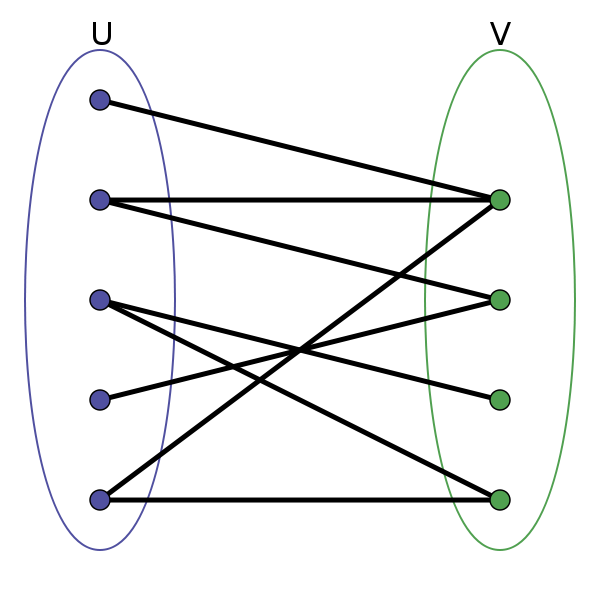
\includegraphics[width=.60\textwidth]{bipartito.png}
\caption{Grafo bipartito}
\end{minipage}
\begin{minipage}[htbp]{.50\textwidth}
\centering
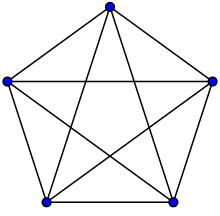
\includegraphics[width=.60\textwidth]{K5.png}
\caption{Grafo completo ($K_{5}$)}
\end{minipage}
\medskip
\begin{minipage}[htbp]{.50\textwidth}
\centering
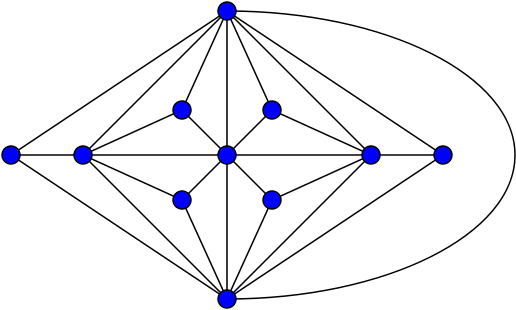
\includegraphics[width=.60\textwidth]{planare.png}
\caption{Grafo planare}
\end{minipage}
\end{figure}

%1.2
\section{Matching e Perfect Matching}
Dato un certo grafo $G$, si vuole trovare quanti pi� archi indipendenti possibili. 

\begin{definizione}
Dato un grafo $G = (V,E)$, un matching ("accoppiamento") $M(G)$ in $G$ � un sottografo di G composto da un insieme di archi a coppie non incidenti, cio� non esistono due archi che condividono un vertice in comune. Oppure, in maniera equivalente, se ogni vertice di G � incidente con al massimo un arco in M, cio� $deg(v)\le 1$ $\forall v\in G$.\\
Questo significa che, in un matching M(G), i vertici possono essere o di grado 1 o 0. In particolare,
\begin{itemize}
\item se deg(v) = 1, allora il vertice v � detto accoppiato (o saturato), cio� v � incidente in uno degli archi in M
\item se deg(v) = 0, allora il vertice v non � accoppiato.
\end{itemize}
In un matching, due archi non sono incidenti: se lo fossero, allora il grado del vertice che collega questi due archi avrebbe grado 2, il che viola la definizione.
\end{definizione}

\begin{figure}[htbp]
\centering
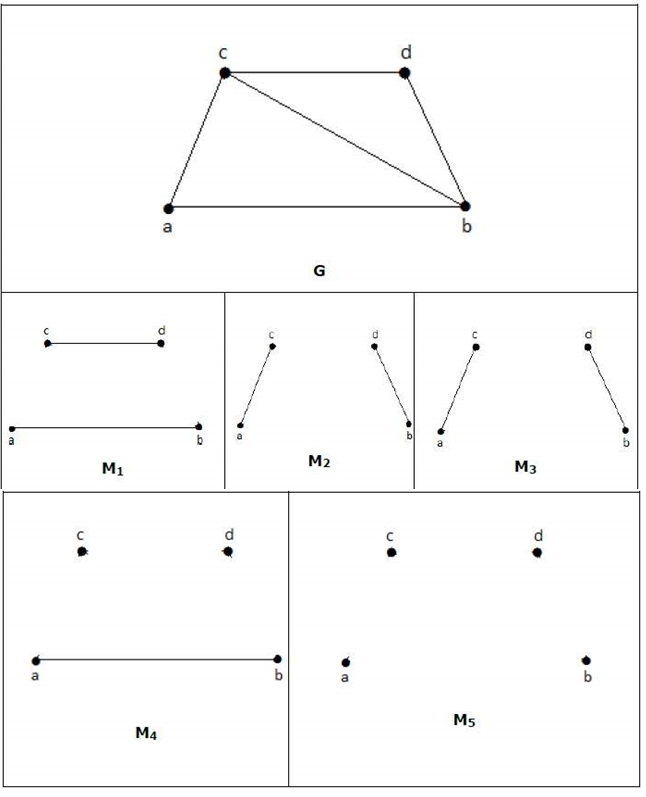
\includegraphics[width=.55\textwidth]{matching.png}
\caption{Esempi di Matching di un grafo G}
\end{figure}


\begin{definizione}
Un grafo $G = (V,E)$ � detto matching massimale se nessun arco di G pu� essere aggiunto ad un matching M. In altre parole, se aggiungiamo un qualsiasi arco (non in M) in M, esso non � pi� un matching.
\end{definizione}

\begin{figure}[htbp]
\centering
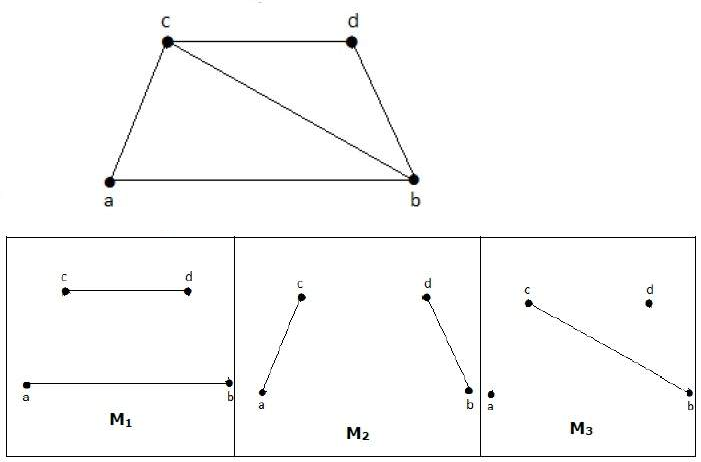
\includegraphics[width=.60\textwidth]{maximal.png}
\caption{$M_{1},M_{2},M_{3}$ sono matching massimale per G}
\end{figure}

\begin{definizione}
Dato un grafo $G = (V,E)$, M(G) � detto matching massimo se M contiene il massimo numero possibile di spigoli. Esso non � unico. Tale numero � detto numero matching. Notare che ogni matching massimo � massimale ma non il viceversa. 
La seguente figura mostra esempi di matching massimi
\end{definizione}

\begin{figure}[htbp]
\centering
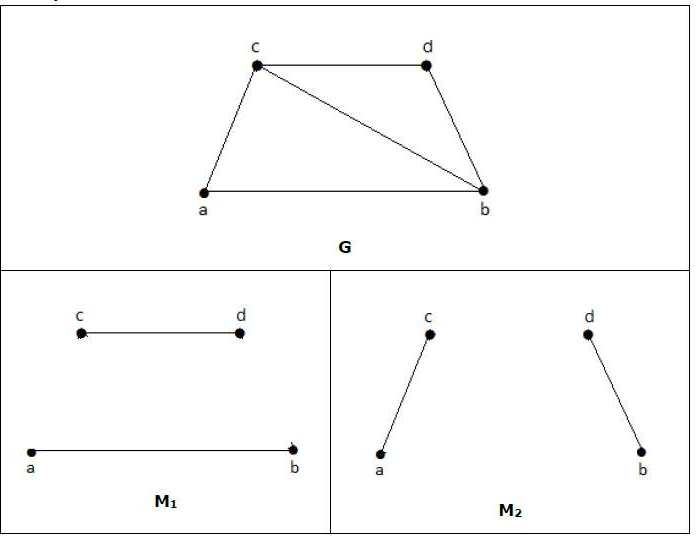
\includegraphics[width=.60\textwidth]{maximum.png}
\caption{$M_{1}$ e $M_{2}$ sono matching massimi per G e il numero matching � 2. Quindi usando il grafo G, possiamo formare solo i sottografi con solo al massimo 2 archi. Per questo abbiamo 2 come numero matching}
\end{figure}

\begin{definizione}
Un matching M(G) di un grafo G � detto perfetto se ogni vertice $v \in G$ � incidente ad un arco $e \in M$, cio� se $deg(v) = 1 \forall v \in V$
\end{definizione}

\begin{figure}[htbp]
\centering
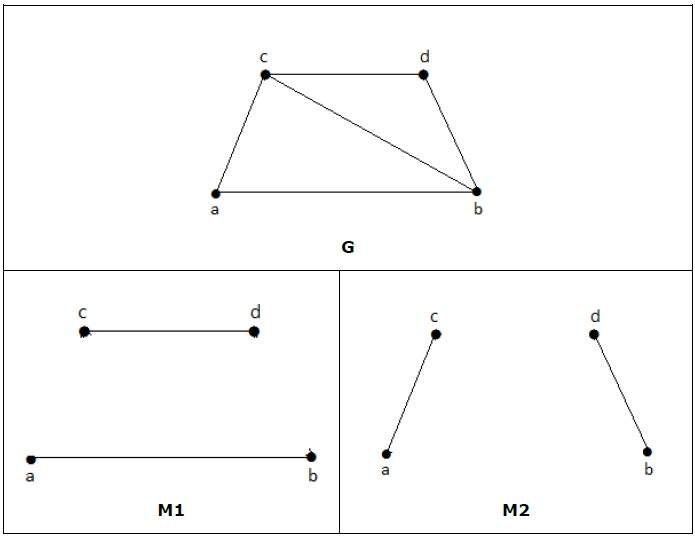
\includegraphics[width=.60\textwidth]{perfect.png}
\caption{$M_{1}$ e $M_{2}$ sono esempi di matching perfetto per G}
\end{figure}

\begin{osservazione}
Dalle definizioni sopra citate si nota che:
\begin{enumerate}
\item Ogni matching perfetto � anche un matching massimo perch� non esiste alcuna possibilit� di aggiungere un altro arco in pi� in un perfect matching. Di conseguenza, � anche massimale;
\item Un matching massimo non � necessariamente perfetto.
\item Se un grafo G ha un matching perfetto, allora il numero di vertici $|V(G)|$ � pari: se fosse dispari, allora l'ultimo vertice si accoppia con un altro e alla fine rimarrebbe un singolo vertice che non � abbinato a nessun altro e quindi avrebbe grado 0. Ma questo non � possibile per definizione di matching perfetto.
\end{enumerate}
\end{osservazione}

\begin{figure}[htbp]
\begin{minipage}[htbp]{.80\textwidth}
\centering
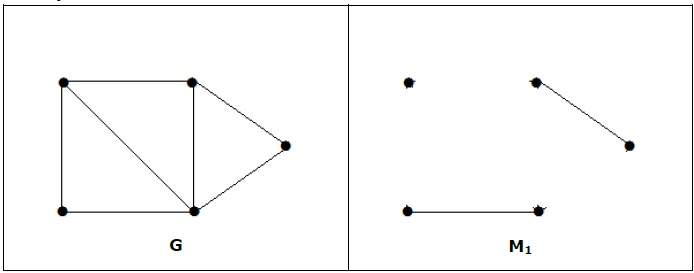
\includegraphics[width=.60\textwidth]{matching1.png}
\caption{Matching non perfetto con un numero dispari di vertici}
\end{minipage}
\begin{minipage}[htbp]{.80\textwidth}
\centering
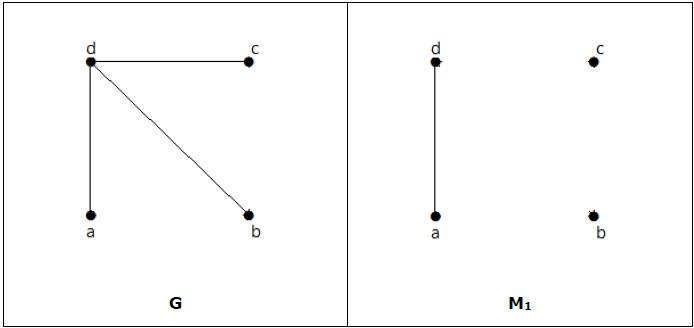
\includegraphics[width=.60\textwidth]{matching2.png}
\caption{E' un matching ma non � perfetto sebbene abbia un numero pari di vertici}
\end{minipage}
\end{figure}

%% 1.3
\section{Alcuni esempi di Perfect Matching}
Per modellare problemi di perfect matching, si utilizzano spesso grafi bipartiti. Si consideri $G = (V,E)$ un grafo bipartito con $\left \{A,B \right \}$ una bipartizione di V, cio� $V = A \cup B$ e $A \cap B = \emptyset$ e tutti archi connettono vertici tra A e B. L'obiettivo � trovare un matching M in G con quanti pi� archi possibili.

Per risolvere alcuni problemi riguardo a possibili combinazioni di cose, si utilizzando questioni e concetti legati alla teoria dei grafi. In questa sezione tratteremo alcuni semplici esempi di perfect matching e vedremo come si risolvono. A questo proposito, enunciamo un risultato importante che sta alla base di molte applicazioni, tra cui l'esempio che seguir�:

\begin{teorema}[Hall, 1935]
Un grafo bipartito $G$ ha un matching $A$ se e solo se
\begin{equation*}
|N(S)| \ge |S| \qquad \forall S \subseteq A
\end{equation*}
\end{teorema}
\begin{proof}
Si veda $[1]$.
\end{proof}

\begin{esempio}
Supponiamo di avere 6 regali (denotati con 1,2,3,4,5,6) da dare a 5 amici (Alice, Bob, Charles, Dot, Edward). La domanda �: posso distribuire un regalo ad ognuno in modo che tutti ottengano quello che desiderano?\\
Certamente, questo dipende dalle preferenze dei singoli amici. Se nessuno di loro piacciono i miei regali allora sono stato sfortunato. Anche se a tutti piacciono alcuni dei doni, non sono in grado di soddisfarli tutti: ad esempio se nessuno ama il regalo 5 o 6, allora avr� solo 4 regali da dare ai 5 amici e quindi il problema non � risolvibile. Escludiamo quindi questi casi. 

\begin{figure}[htbp]
\centering
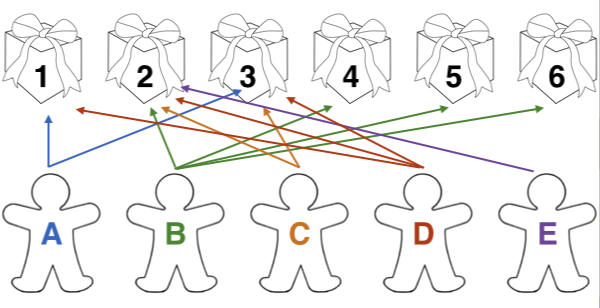
\includegraphics[width=.60\textwidth]{bambini.png}
\caption{Pu� ogni bambino ricevere un regalo che preferisce?}
\end{figure}

Possiamo vedere questa situazione come un grafo partizionato in due insiemi: quello dei regali e quello degli amici. Per definizione, si vede subito che il grafo in questione � bipartito. Ad ogni persona � associato un arco che indica le proprie preferenze sui regali (ad esempio Alice preferisce ricevere il regalo 1 o 3 e cos� via). Verifichiamo se soddisfa o meno il Teorema di Hall: consideriamo come sottoinsieme $X = \left \{ A,C,D,E \right \}$, quindi $|X| = 4$ e di conseguenza $N(X) = \left \{ 1,2,3 \right \}$, quindi $|X| = 3$. Da ci� si evince che $|X| \ge |N(X)|$ pertanto la condizione di Hall non � soddisfatta e quindi non esiste un matching. In altre parole, non � possibile distribuire a tutti il regalo desiderato e quindi accontentare tutti.
\end{esempio}

Un'altro esempio � quello del problema del Vertex Cover. 
\begin{definizione}
Sia $G = (V,E)$ un grafo. Una copertura di vertici di G � un sottoinsieme $U \subseteq V$ tale che ogni arco $e \in E$ � incidente a un vertice  $v \in U$. 
\end{definizione}
Questo � uno dei tanti argomenti sulla teoria dei grafi ed ha molte applicazioni nei problemi di perfect matching e problemi di ottimizzazione. La copertura di vertici pu� essere un buon approccio per un problema dove tutti gli archi di un grafo devono essere inclusi nella soluzione. 
In particolare, spesso viene chiesto di trovare il coprimento con il numero pi� piccolo di vertici. 

\begin{figure}[htbp]
\begin{minipage}[htbp]{.80\textwidth}
\centering
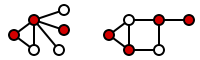
\includegraphics[width=.60\textwidth]{cover.png}
\caption{Esempi di vertex cover segnati in rosso}
\end{minipage}
\begin{minipage}[htbp]{.80\textwidth}
\centering
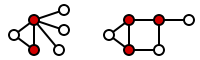
\includegraphics[width=.60\textwidth]{cover1.png}
\caption{Esempi di vertex cover minimo}
\end{minipage}
\end{figure}



\begin{osservazione}
\begin{itemize}
Alcune propriet� del Vertex Cover:
\item L'insieme di tutti i vertici � un coprimento di vertici
\item Gli endpoints di un matching massimale formano un vertex cover
\item Il grafo bipartito completo $K_{m,n}$ ha un vertex cover minimo dato da $min\left \{m,n \right \}$.
\end{itemize}
\end{osservazione}

Il seguente teorema stabilisce una relazione tra vertex cover e perfect matching. In particolare
\begin{teorema}[K\"onig, 1931]
In un grafo G bipartito, il numero di archi di un matching massimale � uguale al numero di vertici in un vertex cover minimo.
\end{teorema}
\begin{proof}
Si veda $[1]$.
\end{proof}

\begin{figure}[htbp]
\centering
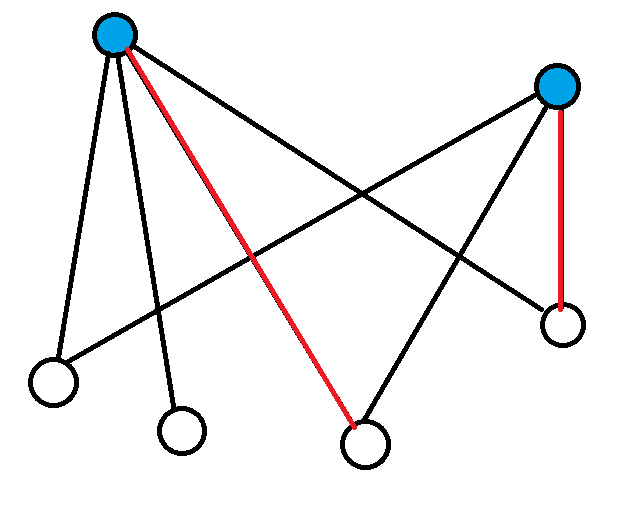
\includegraphics[width=.60\textwidth]{Pm.png}
\caption{Esempio di applicazione del Teorema di K\"onig: i vertici rossi rappresentano il vertex cover minimo mentre gli archi blu indicano un matching massimo}
\end{figure}

In informatica, ci sono algoritmi che implementano questo problema.
\chapter{Algoritmo}
Before explaining all details about the algorithm we developed, we need to introduce some theoretical concept. \\

Consider a graph $G = (V, E)$, defined as a couple of sets: $V$ for vertices, $E$ for edges; $\delta_{G}(S)$ (or $\delta(S)$) is the set of those edges in $E$ with precisely one end-vertex in $S$, subset of $V$. We define a \emph{graft} $(G,T)$ as a connected graph $G$\footnote{A graph $G = (V,E)$ is said \emph{connected} if, for all pairs $(u,v) \in V$ there exists a path between them. A maximal connected subgraph of an undirected graph is said \emph{connected component} of the graph.} in which an even number of vertices $T \subseteq V$ have been distinguished as \emph{odd}. The \emph{T-parity} of a set of vertices $S \subseteq V$ is the parity of $|S \cap T|$. When $S \subseteq V$ is $T$-odd then $\delta(S)$ is a \emph{T-odd cut} or \emph{T-cut}. \\
  
 In order to make a complete description of the algorithm developed, consider the following concept: the \textbf{Gomory-Hu tree}\footnote{Recall that an acyclic graph is a \emph{forest} and a connected forest is a \textbf{tree}} of an undirected graph, i.e. a graph without orientation, is a weighted tree that represents the minimum $\{s,t\}$-cuts for all $\{s,t\}$ pairs in the graph. The Gomory-Hu tree can be constructed in $|V| - 1$ maximum flow computations.
 
 \begin{definition}
 Let $G = ((V_G, E_G), c)$ be an undirected graph with $c(u,v)$ being the capacity of the edge $(u,v)$ respectively. Denote the minimum capacity of an $\{s,t\}$-cut by $\lambda_{s,t}$ for each $\{s,t\} \in V_G$. Let $T = (V_T, E_T)$ be a tree with $V_T = V_G$, denote the set of edges in an $\{s,t\}$ path by $P_{s,t}$ for each $\{s,t\} \in V_T$. Then $T$ is said to be a \textbf{Gomory-Hu tree} of $G$ if
 \[
 \lambda_{s,t} = \min_{e \in P_{s,t}} c(S_e, T_e) \quad \text{for all} \quad \{s,t\} \in V_{G},
 \]
 where
 \begin{enumerate}
 \item $S_e$ and $T_e$ are the two connected components of $T \setminus \{e\}$ in the sense that $(S_e, T_e)$ forms a $s,t$-cut in G. \\
 \item $c(S_e, T_e)$ is the capacity cut in G.
 \end{enumerate}
 \end{definition}
Let $(G,T)$ be a graft and $c: E \to \R_+$ be a \emph{cost} function. A minimum $T$-cut for $(G,T,c)$ is a $T$-cut $\delta(X)$ of $(G,T)$ for which:
\[
c(\delta(X)) = \lambda_{G,T} = \min\{c(\delta(S)): \delta(S)\quad \text{is a $T$-cut of}\quad(G,T) \}
\]
where the cost $c(F)$ of a set $F$ of edges is defined as $\sum_{e \in F} c(e)$.
In particular, we recall some basic facts about submodularity and uncrossing. The complement in $V$ of $S \subseteq V$ is denoted by $\bar{S} = V \setminus S$. \emph{Switching} $S$ means replacing $S$ by $\bar{S}$. For example, if $S = X$, then after switching $S$ we obtain that $S = \bar{X}$ and $\bar{S} = X$. \\
Let $(G, T)$ be a graft and $S \subseteq V$ a set of nodes. 

\begin{observation}
Switching S does not change the $T$-parity of a $S$ (nor  $\delta(S)$), since $|S \cap T|$ and $|\bar{S} \cap T|$ have the same parity since $|T|$ is even.
\end{observation}

\begin{proposition}
Let (G,T) be a graft and $S, X \subseteq V$. Then we have: 
\begin{enumerate}
\item Switching S change the $T$-parity of $S \cap X$ if and only if $X$ is T-odd.\\
\item $S \cap X$ and $S \cup X$ have the same $T$-parity if and only if $S$ and X have the same T-parity. \\
\item Switching S changes the T-parity of $S \cup X$ if and only if X is T-odd.
\end{enumerate}
\end{proposition}

\begin{proof}
Note that $|(S \cap X) \cap T| = |S \cap (X \cap T)|$ whose parity is affected by switching $S$ if and only if $|X \cap T|$ is odd, that is, if and only if $X$ is $T$-odd. This gives $(1)$. To obtain $(2)$ note that $|(S \cap X) \cap T| + |(S \cup X) \cap T| = |S \cap T| + |X \cap T|$. Finally, $(3)$ is a consequence of $(1)$ and $(2)$.
\end{proof}

The following lemma expresses a property of cuts known as \emph{submodularity}.
\begin{lemma}
Let G be a graph with cost function $c: E \longmapsto \R_+$. Let $S_{1}, S_{2} \subseteq V$.
\begin{equation}
c(\delta(S_{1} \cap S_{2})) + c(\delta(S_{1} \cup S_{2})) \leq c(\delta(S_1)) + c(\delta(S_2))
\end{equation}
\end{lemma}

\begin{proof}
We claim that each edge $uv$ contributes to the right at least as to the left side of (2.1). By Proposition 2.2, if $S_1 \cap S_2$ have different $\{u,v\}$-parities, so do $S_1$ and $S_2$. Hence, had our claim to be false, then both $S_1 \cap S_2$ and $S_1 \cup S_2$ would be $\{u,v\}$-odd. Assume w.l.o.g. that $u \in S_1 \cup S_2$ and $u \notin S_1 \cup S_2$. Then, $u \in S_1, S_2$ and $u \notin S_1, S_2$
\end{proof}

If $S \cap X \neq \O$ for every possible switching of $S$ and $X$, then $S$ and $X$ are said to \emph{cross}. All what we will need about cut functions is that they obey to the following lemma. 

\begin{lemma}
Let $T_{1}, T_{2}$ be even cardinality subsets of V. Let $\delta(S_1)$ be a minimum $T_1$-cut and assume that $S_1$ is $T_2$-even. Then there exists a minimum $T_2$-cut $\delta(S_2)$ such that $S_1$ and $S_2$ do not cross.
\end{lemma}

\begin{proof}
Let $\delta(X)$ be a minimum $T_2$-cut. We remark that, by Proposition 2.2, switching $S_1$ changes the $T_2$-parity of $S_1 \cup X$ whereas switching $X$ changes the $T_1$-parity of $S_1 \cap X$ leaving the $T_2$-parity of $S_1 \cup X$ unaffected. Therefore, by possibly switching $S_1$, we can assume that $S_1 \cup X$ is $T_2$-odd. Afterwards, by possibly switching $X$, we can assume that $S_1 \cap X$ is $T_1$-odd without affecting the $T_2$-parity of $S_1 \cup X$. 
At this point, $c(\delta(S_1 \cup X)) \ge c(\delta(S_1))$ since $\delta(S_1)$ is a minimum $T_1$-cut. By sub-modularity, $c(\delta(S_1 \cup X)) = c(\delta(X))$. Thus, $\delta(S_1 \cup X)$ is a minimum $T_2$-cut. And clearly, $S_1$ and $S_1 \cup X$ do no cross. 
\end{proof}

\section{Minimum $T$-cuts: a simple algorithm}
Now, we will present an algorithm for $T$-cut. Consider a graft $(G,T)$ and a $T$-even set $S \subseteq V$, denoted by $G_S$ the graph obtained from $G$ by identifying all nodes in $S$ into a single node and letting $T_S := T \setminus S$. Note that $(G_S, T_S)$ is a graft. When $S = \{ s, t \} \subseteq T$ then we rely on a shorter notation $G_{s,t} = G_{\{s,t\}}$ and $T_{s,t} = T_{\{s,t\}}$. \\
Since node identification does not affect the edge set of a graph, a cost function $c$ for $G$ is also a cost function for $G_S$ and $G_{s,t}$.
Then, we show four steps to compute $\lambda_{G,T}$:\\

\texttt{MinT-cut(G,T,c)}
\begin{enumerate}
\item if $T = \O$ then return $\infty$, that means $(G,T)$ does not contains any $T$-cut;\\
\item let $s$ and $t$ be any two different nodes in $T$; \\
\item let $\delta(S)$ be a minimum $\{s,t\}$-cut; \\
\item if $S$ is $T$-odd then return $\min( c(\delta(S)), \texttt{MinT-cut($G_{s,t}, T_{s,t}$, c)})$; otherwise return $\min(\texttt{MinT-cut($G_{S}, T_{S}$, c)}; \texttt{MinT-cut($G_{\bar{S}}, T_{\bar{S}}$, c)})$
\end{enumerate}

\section{Correctness}
For a given $(G,T,c)$, let $s$ and $t$ be any two different nodes in $T$ and let $\delta(S)$ be a minimum $\{s,t\}$-cut. The correctness of the above procedure relies on the following two lemmas:
\begin{lemma}
If $\delta(S)$ is T-odd, then $\lambda_{G,T} = \min(c(\delta(S)), \lambda_{G_{s,t}, T_{s,t}})$.
\end{lemma}

\begin{proof}
Indeed, the $T_{s,t}$-cuts of $G_{s,t}$ are precisely the $T$-cuts of $G$ that are not $\{s,t\}$-odd.
\end{proof}

\begin{lemma}
If $\delta(S)$ is T-even, then $\lambda_{G,T} = \min( \lambda_{G_{S}, T_{S}}, \lambda_{G_{\bar{S}}, T_{\bar{S}}})$.
\end{lemma}

\begin{proof}
First note that every $T_S$-cut in $(G_S, T_S)$ and every $T_{\bar{S}}$-cut in $(G_{\bar{S}},T_{\bar{S}})$ is also a $T$-cut in $(G,T)$. This implies $\lambda_{G,T} \le \min( \lambda_{G_{S}, T_{S}}, \lambda_{G_{\bar{S}}, T_{\bar{S}}})$. 
For the converse, let $\delta(X)$ be any minimum $T$-cut for $(G,T,c)$. By Lemma 2.4, we can assume that $S$ and $X$ do not cross. This means that the edge set $\delta_{G}(X)$ is either a $T_S$-cut in $G_S$ or a $T_{\bar{S}}$-cut in $G_{\bar{S}}$.
\end{proof}

\section{Computing optimal $T$-parings}
Let $(G,T)$ be a graft with cost function $c: E \longmapsto \R_+$. A \emph{T-pairing} is a partition of $T$ into pairs. The value of the $T$-pairing $\mathcal{P}$ is defined as: 
\[
val_G (\mathcal{P}) = \min_{\{u,v\} \in \mathcal{P}} \lambda_{G}(u,v) 
\]
where $\lambda_G (u,v)$ denotes the cost of a minimum $\{u,v\}$-cut, Let $\mathcal{P}$ be any $T$-pairing and $\delta(S)$ be any $T$-cut. Since $\delta(S)$ is $T$-odd, $\mathcal{P}$ contains a pair $\{u,v\}$ such that $\delta(S)$ is $\{u,v\}$-odd. Therefore, $c(\delta(S)) \ge \lambda_G (u,v) \ge val_G (\mathcal{P})$ and the value of $\mathcal{P}$ is a lower bound on $\lambda_{G,T}$.\\
In this section, we show that the algorithm \emph{MinT-cut} actually finds a $T$-pairing of value $\lambda_{G,T}$. Indeed, consider a single iteration of the algorithm. Let $s$ and $t$ be two odd nodes. Let $\delta(S)$ be a minimum $\{s,t\}$-cut. 

\begin{lemma}
Let $\delta(S)$ be a minimum $\{s,t\}$-cut in $(G,c)$. Then we have: 
\[
\lambda_G (u,v) \ge \min(c(\delta(S)), \lambda_{G_{s,t}}(u,v)) \qquad \forall u,v \in V(G) \setminus \{s,t\}
\]
\end{lemma}

\begin{proof}
Indeed, the $\{u,v\}$-cuts of $G_{s,t}$ are exactly the $\{u,v\}$-cuts of $G$ that are not $\{s,t\}$-odd.
\end{proof}

\begin{lemma}
Let $\delta(S)$ be a minimum $\{s,t\}$-cut in $(G,c)$. Then we have: 
\[
\lambda_G (u,v) = \lambda_{G_{s}} (u,v) \qquad \forall u,v \in V(G) \setminus S
\]
\end{lemma}

\begin{proof}
Let $u$ and $v$ be two any nodes in $V(G) \setminus S$. Obviously $\lambda_G (u,v) \le \lambda_{G_{s}} (u,v)$. For the converse, let $\delta(X)$ be any minimum $\{u,v\}$-cut in $G$. By Lemma 2.4, we can assume that $S$ and $X$ do not cross. Then, the edge set $\delta_{G}(X)$ is a $\{u,v\}$-cut in $G_S$ and $\lambda_G (u,v) = \lambda_{G_{s}} (u,v)$.
\end{proof}

Each iteration of the algorithm contemplates two possibilities: 
\begin{enumerate}
\item \textbf{Case 1}: $\delta(S)$ is $T$-odd. By Lemma 2.5, $\lambda_{G,T} = \min\{c(\delta(S)), \lambda_{G_{s,t},T_{s,t}}\}$. By Lemma 2.7, if $\mathcal{P'}$ is a $T_{s,t}$-pairing with $val_{G_{s,t}}(\mathcal{P'}) = \lambda_{G_{s,t},T_{s,t}}$, then $\mathcal{P} = \mathcal{P'} \cup \{s,t\}$ is a $T$-pairing with $val_{G} (\mathcal{P}) \ge \min(c(\delta(S)), val(\mathcal{P'})) = \min(c(\delta(S)), \lambda_{G_{s,t},T_{s,t}}) = \lambda_{G,T}$. \\
\item \textbf{Case 2}: if $\delta(S)$ is $T$-even. By Lemma 2.6, $\lambda_{G,T} = \min\ \lambda_{G_{S},T_{S}}, \lambda_{G_{\bar{S}},T_{\bar{S}}}\}$. By Lemma 2.8, if $\mathcal{P_S}$ is a $T_{S}$-pairing with $val_{G_{S}} (\mathcal{P_S}) = \lambda_{G_{S},T_{S}}$ and $\mathcal{P_{\bar{S}}}$ is a $T_{\bar{S}}$-pairing with $val_{G_{\bar{S}}} (\mathcal{P_{\bar{S}}}) = \lambda_{G_{\bar{S}},T_{\bar{S}}}$ then $\mathcal{P} = \mathcal{P_S} \cup \mathcal{P_{\bar{S}}}$ is a $T$-pairing with $val_{G} (\mathcal{P}) \ge \min(val(\mathcal{P_S}), val(\mathcal{P_{\bar{S}}})) = \min(\lambda_{G_{S},T_{S}}\lambda_{G_{\bar{S}},T_{\bar{S}}}) = \lambda_{G,T}$.
\end{enumerate}  

The following results summarize this section. 

\begin{theorem}
For every $(G,T,c)$ the maximum value of a $T$-pairing equals the minimum cost of a T-cut.
\end{theorem}

\begin{theorem}
For every node u in T there exists a node $v \in T \setminus \{u\}$ such that $\{u,v\}$ is useful.
\end{theorem}

\begin{proof}
Apply algorithm \emph{MinT-cut} to $(G,T,c)$. At each recursion, keep choosing $s = u$ until the minimum $\{s,t\}$-cut $\delta(S)$ is $T$-odd. By Lemma 2.8, $\{u,v\}$ is useful w.r.t. $(G,T,c)$.
\end{proof}

\section{Algorithm}
We have developed an algorithm on Python using both Gurobi and Python languages. It can be run using Spyder\footnote{It is in Anaconda.}(full code is in Appendix A). In what follows, we analyze the main aspects of the algorithm. It is composed of two parts: 
\begin{enumerate}
\item In the first part, we gave four important functions: \texttt{Contraction}, \texttt{minCutValue}, \texttt{findsubsets} and \texttt{minCutEdges};\\
\item After that,  we developed the model (constraint and objective function). The final \texttt{while} cycle optimize the model. 
\end{enumerate}

We start analyzing the second part of the code. First, we create the variables: we define a lower bound at zero and consider them continuous as type. At the beginning, we defined them as binary variable, but in this way we always found an integer solution. So in order to solve a real problem (i.e. non integer solution), we have decided to change the variables type as continuous. In this case, at first we obtain a non-integer solution. 
Then we add the objective function: 
\[
\min \sum_{ij} \texttt{edges} \cdot \texttt{var}
\]
that minimizes the sum of all products between the continuous variable \texttt{var} and \texttt{edges} which represents the cost value of the considered edge. The only constraint we consider: the sum of all edges entering in a certain vertex must be 1. \\
After looking for edges incident to a vertex $i$ and after building up the constraint we explained before, we define the optimization model. We iteratively make the code looking for integer solution thanks to a while-cycle. This means that, in the cycle, it optimizes the model, then it finds the value of minimal odd cut and checks if this value is less or greater than 1. \\
If the minimal odd cut is less than 1, it finds the edges of the minimal odd cut and adds a constraint, that is the sum of the variables associated to the edges of the minimal cut have to be greater or equal to 1.  And so on, until it finds an integer solution. \\

In the first part of the code, we import firstly the useful modules we need to develop the optimization model. This part is based on finding minimum $T$-cut.
We define a function for contraction, which at the end creates a minor of $G$. Then, the function \texttt{minCutValue(graph, T)} finds the value of minimum odd cut  of a given graph; \texttt{T} is a datum used during the recursion: it must be initially set equal to '\texttt{vertices}'. The third function we define is \texttt{findsubset}, which finds all subsets of a fixed cardinality of a given set. Given a graph and the value of one of its minimum odd cuts, we construct a function which finds the edges of the minimum odd cut \texttt{minCutEdges}.   \\

In another file Python we have considered some graphs on which test the algorithm, such as Petersen graph, TSP problem, an unfeasible graph (i.e. a graph which has not a perfect matching) and $K(5)$ graph which are described in Appendix B. 

\chapter{Conclusione}
Nonostante i vantaggi dell'algoritmo presentato, il codice pu� essere migliorato. Per esempio, si possono fare le seguenti modifiche:
\begin{itemize}
\item I dizionari (.keys all'interno del codice) potrebbero essere usati per i vertici e non per gli archi, ma in questo caso si dovrebbe risolvere il problema dei pesi da assegnare agli archi;
\item Gli esempi sono stati inseriti in un file python a parte e si potrebbe riuscire a strutturarlo come file di testo e richiamarlo nel file python matching;
\end{itemize}

L'idea iniziale era quella di utilizzare le funzioni Call-Back, cio� di utilizzarla all'interno del ciclo while come nel caso del TSP (Problema del commesso viaggiatore). In questo caso, tuttavia, le funzioni Call-Back non si potevano usare in quanto Gurobi non permette all'utente di utilizzare il valore delle variabili se non nella fase MIP, cio� in una fase del processo in cui si hanno solo valori interi delle soluzioni, ma il problema che si vuole aggirare con questo algoritmo � proprio quello di usare solo valori interi delle soluzioni.

Si � giunti quindi ad una contraddizione e si � dovuta scartare l'idea di utilizzare Call-Back all'interno del codice.

In conclusione, l'algoritmo pu� essere migliorato ed � stato aggirato il problema di utilizzare un certo tipo di funzioni all'interno del codice a causa di restrizioni del programma.

\appendix
\chapter{Perfect-Matching Codice}
\begin{verbatim}
@author: Alessandro Zeggiotti
# -------------------------------------------------------------------
# USEFUL MODULES

import math
import random
from gurobipy import *

import networkx as nx
import itertools

# Matching_examples.py contains some useful examples to test this script
# QUESTION: Is "import" the best way to run an external script?
from Matching_examples import *

# -------------------------------------------------------------------
# FUNCTIONS DEFINITION

# Given a graph, this function idefintifies a set of nodes into a single vertex

def Contraction(graph, nodes):
    V = set()
    for i,j in graph:
        V = V.union({i})
        V = V.union({j})
    new_vertex = max(V) + 1
    # Create a minor of the graph
    minor = {}
    for i,j in graph.keys():
        if i in nodes and j in nodes:
            pass
        elif i in nodes and (j,new_vertex) not in minor.keys():
            minor[j,new_vertex] = graph[i,j]
        elif i in nodes:
            minor[j,new_vertex] += graph[i,j]
        elif j in nodes and (i,new_vertex) not in minor.keys():
            minor[i,new_vertex] = graph[i,j]
        elif j in nodes:
            minor[i,new_vertex] += graph[i,j]
        else:
            minor[i,j] = graph[i,j]
    return minor

# Given a graph, this function finds the value of a minimum odd cut
# T is a datum used during the recursion: 
#it must be initially set equal to "vertices"

def minCutValue(graph, T):
    # Base step
    if T == set():
        return float('inf')
    # Create the graph using the module NETWORKX
    G = nx.DiGraph()
    for (i,j) in graph.keys():
        G.add_edge(i, j, capacity = graph[i,j])
        G.add_edge(j, i, capacity = graph[i,j])
    # Let s and t be two random nodes in T
    s = min(T)
    t = max(T)
    # NETWORKX contains a function that allows to find the minimum s-t cut
    # This function is based on Ford-Fulkerson algorithm
    cut_value, partition = nx.minimum_cut(G,s,t)
    S, S_bar = partition
    if len(S.intersection(T)) % 2 == 1: # if S is T-odd: ...
        return min(cut_value,
                   minCutValue(Contraction(graph, {s,t}), T - {s,t}))
    else:
        return min(minCutValue(Contraction(graph, S), T - S),
                   minCutValue(Contraction(graph, S_bar), T - S_bar))

# Given a set, this function finds all its subsets of a fixed cardinality

def findsubsets(S,m):
    # From ITERTOOLS module
    return set(itertools.combinations(S, m))

# Given a graph and the value of a minimum odd cut, 
# this function finds a minimum odd cut

def minCutEdges(graph, cut_value):
    for cardinality in range(1,n,2):
        subsets = findsubsets(vertices, cardinality) 
        # "vertices" is global variable
        for S in subsets:
            # Create the cut
            dS = {}
            for i,j in graph.keys():
                if i in S and j not in S:
                    dS[i,j] = graph[i,j]
                if i not in S and j in S:
                    dS[i,j] = graph[i,j]
            dS_value = sum(dS.values())
            if dS_value == cut_value:
                return dS
    print('No odd cut of value %g has been found' % cut_value)
    return None

# -------------------------------------------------------------------
# MODEL DEFINITION

m = Model()
# Suppress the standard output, it would be invoked too many times
m.setParam('OutputFlag', 0)

# Create the variables
vars = {}
for (i,j) in edges.keys():
   vars[i,j] = m.addVar(lb=0, vtype=GRB.CONTINUOUS, name='e[%d,%d]'%(i,j))

# To create the model data structure only once, after variables creation
m.update()

# Add the objective function
m.setObjective(sum(vars[i,j]*edges[i,j] for i,j in edges.keys()), GRB.MINIMIZE)

# Add degree-1 constraint
for i in vertices:
    # Look for the edges incident to i
    neighbors = []
    for j in vertices:
        if (i,j) in edges.keys():
            neighbors.append((i,j))
        elif (j,i) in edges.keys():
            neighbors.append((j,i))
    m.addConstr(sum(vars[i,j] for i,j in neighbors) == 1)

# -------------------------------------------------------------------
# MODEL OPTIMIZATION

linked = set()
for edge in edges.keys():
    linked = linked.union(set(edge))

# Check the presence of isolated vertices
if vertices != linked:
    print(str(vertices - linked) + ' is a set of isolated vertices!')

# Check the parity of the graph
elif n % 2 == 1:
    print('The graph is odd!')

else:
    # Now we are sure that the graph admits a solution
    while True:
        # Solve the problem
        m.optimize()
        print('\n--------------------------------------------------------\n')
        solution = m.getAttr('x', vars)
        selected = [(i,j) for i,j in solution.keys() if solution[i,j] != 0]
        print('New incumbent solution:\n')
        for i,j in selected:
            print('    ' + str((i,j)) + ' : ' + str(solution[i,j]))
        print('\nObjective function: %g' % m.objVal)
        print('Checking the presence of rationals...')
        # Find the value of a minimum odd cut
        cut_value = minCutValue(solution, vertices)
        if cut_value < 1:
            # Find the edges of a minimum odd cut
            cut_edges = minCutEdges(solution, cut_value)
            # Add a constraint
            m.addConstr(sum(vars[i,j] for (i,j) in cut_edges.keys()) >= 1)
            print('Minimum odd cut: %g' % cut_value)
            print('Related edges:\n')
            for i,j in cut_edges.keys():
                print('    ' + str((i,j)) + ' : ' + str(cut_edges[i,j]))
            print('\nNew constraint added...')
        else:
            print('This is a feasible solution!')
            break
\end{verbatim}
\chapter{Perfect-Matching Code Esempi}
\begin{verbatim}
@author: Alessandro Zeggiotti
"""

# Create vertices and edges for our example
# The user can choose one among the four following graphs
print('\n1 --> TSP problem')
print('2 --> Petersen graph')
print('3 --> Unfeasible graph')
print('4 --> K(5)')
choice = int(input('Choose your favourite example: '))

if choice == 1:
    vertices = {0,1,2,3,4,5}
    edges = {
        (0,1): 5,
        (0,2): 5,
        (0,3): 4,
        (1,4): 2,
        (1,5): 3,
        (2,3): 3,
        (2,5): 8,
        (3,4): 4,
        (4,5): 4}
elif choice == 2:
    vertices = {0,1,2,3,4,5,6,7,8,9}
    edges = {
        (0,1): 1,
        (0,4): 1,
        (0,5): 1,
        (1,2): 1,
        (1,6): 1,
        (2,3): 1,
        (2,7): 1,
        (3,4): 1,
        (3,8): 1,
        (4,9): 1,
        (5,7): 1,
        (5,8): 1,
        (6,8): 1,
        (6,9): 1,
        (7,9): 1}
elif choice == 3:
    vertices = {0,1,2,3}
    edges = {
        (0,2): 1,
        (0,3): 1,
        (2,3): 1}
else:
    vertices = {0,1,2,3,4}
    edges = {
        (0,1): 1,
        (0,2): 1,
        (0,3): 1,
        (0,4): 1,
        (1,2): 1,
        (1,3): 1,
        (1,4): 1,
        (2,3): 1,
        (2,4): 1,
        (3,4): 1}

n = len(vertices)


\end{verbatim}

\begin{thebibliography}{90}        
%\begin{enumerate}[{[K1]}]
\bibitem{K1} Reinhard Diestel, "Graph Theory", Electionic Edition 2005
\bibitem{K2} John M. Harris, Jeffry L. Hirst, Michael J.Mossinghoff, "Combinatorics and Graph Theory", Springer Edition 2008
\bibitem{K3} Romeo Rizzi, "A Simple Minimum T-Cut Algorithm", October 23, 2002
%\end{enumerate}
\end{thebibliography}
\end{document}
